\documentclass[11pt]{article}

\usepackage[a4paper,margin=1in]{geometry}
\usepackage{graphicx}
\usepackage{booktabs}
\usepackage{longtable}
\usepackage{csvsimple}
\usepackage{caption}
\usepackage{float}
\usepackage{hyperref}

\hypersetup{
  colorlinks=true,
  linkcolor=black,
  urlcolor=blue,
  citecolor=black
}

\newcommand{\StudentName}{Ethan Benchetrit, Lorenzo Marasco}
\newcommand{\PaperTitle}{How energy prices shape OECD economic growth: Panel evidence}
\newcommand{\PaperAuthors}{Huntington and Liddle}
\newcommand{\PaperYear}{2022}
\newcommand{\PaperJournal}{Energy Economics}
\newcommand{\PaperVolume}{111}
\newcommand{\PaperPages}{106082}
\newcommand{\PaperDOI}{10.1016/j.eneco.2022.106082}

\title{Panel Data Replication Report}
\author{\StudentName}
\date{May 2026}

\begin{document}
\maketitle

\section*{Reference and data}
\textbf{APA reference.} \PaperAuthors\ (\PaperYear). \PaperTitle. \textit{\PaperJournal}, \PaperVolume, \PaperPages. \url{https://doi.org/\PaperDOI}

\textbf{Link to the paper.} \url{https://doi.org/\PaperDOI}

\textbf{Data used.} The replication uses the author-provided dataset \texttt{growth_EE.xlsx} (included in this repository). The dataset contains macroeconomic variables used in the paper. Any data source details follow the paper and the accompanying spreadsheet documentation.

\textbf{Formatted datasets.} The same dataset was prepared for Python, Stata, and R workflows. The Python pipeline is in \texttt{replication_final.py}. The Stata and R translations are in \texttt{replication.do} and \texttt{replication.R}.

\textbf{LLM translation difficulties (R and Stata).}
\begin{itemize}
  \item No official R package provides \texttt{xtdcce2}; CCEMG must be coded manually.
  \item Pesaran CIPS and delta tests are not in \texttt{plm} and require manual or external implementation.
  \item Panel IV estimation per country is not native in \texttt{plm}; \texttt{ivreg} loops are needed.
  \item Panel IRFs and some robustness steps require manual post-estimation code.
\end{itemize}

\section*{Abstract (about 100 words)}
This report partially replicates Huntington and Liddle (2022) on the effect of energy prices on OECD growth. Using the author-provided dataset for 18 OECD countries over 1960--2016 (with a baseline sample from 1972), I reproduce the main descriptive statistics, unit-root tests, cross-section dependence tests, and the core CCE-MG estimates with robustness checks. I also estimate static panel models (between, within, Mundlak, TWFE, first differences) and dynamic ARDL specifications with Anderson--Hsiao IV. The results confirm a negative short-run energy price effect and show heterogeneous responses across countries.

\section*{Introduction (summary of new insights)}
Three replication-based insights stand out. First, energy-price effects on growth are heterogeneous across countries, and this heterogeneity is visible even before imposing a common slope model. Second, first-difference stationarity is strong for all core variables, while levels show weaker evidence, reinforcing the use of differenced specifications. Third, robustness checks (Great Moderation split, recession dummy, country exclusions) yield similar qualitative results, suggesting that the negative short-run effect of energy prices is not driven by single episodes or outliers.

\section*{Table 1: Key correlation of the paper}
\textbf{Dependent variable (Y).} Real GDP (log level) and its first difference (growth).

\textbf{Key explanatory variable (X).} Energy prices (log level) and its first difference.

\textbf{Level.} Country-year panel (OECD countries).

\textbf{Links to data.} This replication uses the author-supplied dataset; source links are documented in the paper and in the Excel workbook metadata.

\section*{Database update}
No update to post-2016 data was attempted in this replication. The dataset remains as provided by the authors. If updates are added later, the same pipeline can be rerun to regenerate all outputs.

\section*{Panel data sample selection}
The full dataset includes 18 countries with a maximum span from 1960 to 2016. All countries have at least three consecutive observations of the dependent variable, so no unit is excluded for the dynamic panel requirement. The panel is slightly unbalanced due to a shorter time span for Australia and Germany.

\textbf{Individuals excluded:} None.

\textbf{Panel size summary:} 18 countries; unbalanced; maximum $T=57$ for most countries.

\subsection*{Number of individuals per date}
\csvautotabular{outputs/obs_by_year.csv}

\subsection*{Number of individuals by their time observations}
\begin{tabular}{ll}
\toprule
Observations per country & Number of countries \\
\midrule
57 & 16 \\
55 & 1 \\
45 & 1 \\
\bottomrule
\end{tabular}

\section*{Panel data variable classification}
The within-variance share is reported below. No variable is fully time-invariant in this dataset. The ordering shows that CPI and energy prices have high within variation, while government expenditure and trade openness have lower within shares.

\csvautotabular{outputs/descriptive_variance.csv}

\section*{Descriptive statistics and tests}
\subsection*{Table 1: Data summary}
\csvautotabular{outputs/table1_data_summary.csv}

\subsection*{Table 2: CIPS unit-root tests}
\csvautotabular{outputs/table2_cips_unitroot.csv}

\subsection*{Cross-section dependence tests (Pesaran CD)}
\csvautotabular{outputs/cd_tests.csv}

\subsection*{Slope heterogeneity (Pesaran--Yamagata delta test)}
\csvautotabular{outputs/delta_test.csv}

\section*{Static panel estimators}
The following table reports between, within, Mundlak (random effects with means), two-way fixed effects, and first-difference estimators.

\csvautotabular{outputs/panel_models_table.csv}

\section*{CCE-MG estimates and robustness}
\subsection*{Table 3: CCE-MG baseline and robust estimates}
\csvautotabular{outputs/table3_cce_robust.csv}

\subsection*{Table 4: CCE-MG robustness checks}
\csvautotabular{outputs/table4_ccemg_robustness.csv}

\subsection*{Table 5: Country responses and energy intensity}
\csvautotabular{outputs/table5_country_responses.csv}

\subsection*{Table 6: Country responses and intensity regressions}
\csvautotabular{outputs/table6_intensity_regression.csv}

\section*{Dynamic ARDL and Anderson--Hsiao IV}
\subsection*{ARDL (OLS)}
\csvautotabular{outputs/ardl_ols.csv}

\subsection*{ARDL (IV)}
\csvautotabular{outputs/ardl_iv.csv}

\subsection*{First-stage R2 (IV)}
\csvautotabular{outputs/first_stage_r2.csv}

\subsection*{Hausman test (OLS vs IV)}
\csvautotabular{outputs/hausman_ols_iv.csv}

\subsection*{Impulse response (energy price shock)}
\csvautotabular{outputs/irf.csv}

\subsection*{Long-run effect}
\csvautotabular{outputs/long_term.csv}

\section*{Figures}
\begin{figure}[H]
  \centering
  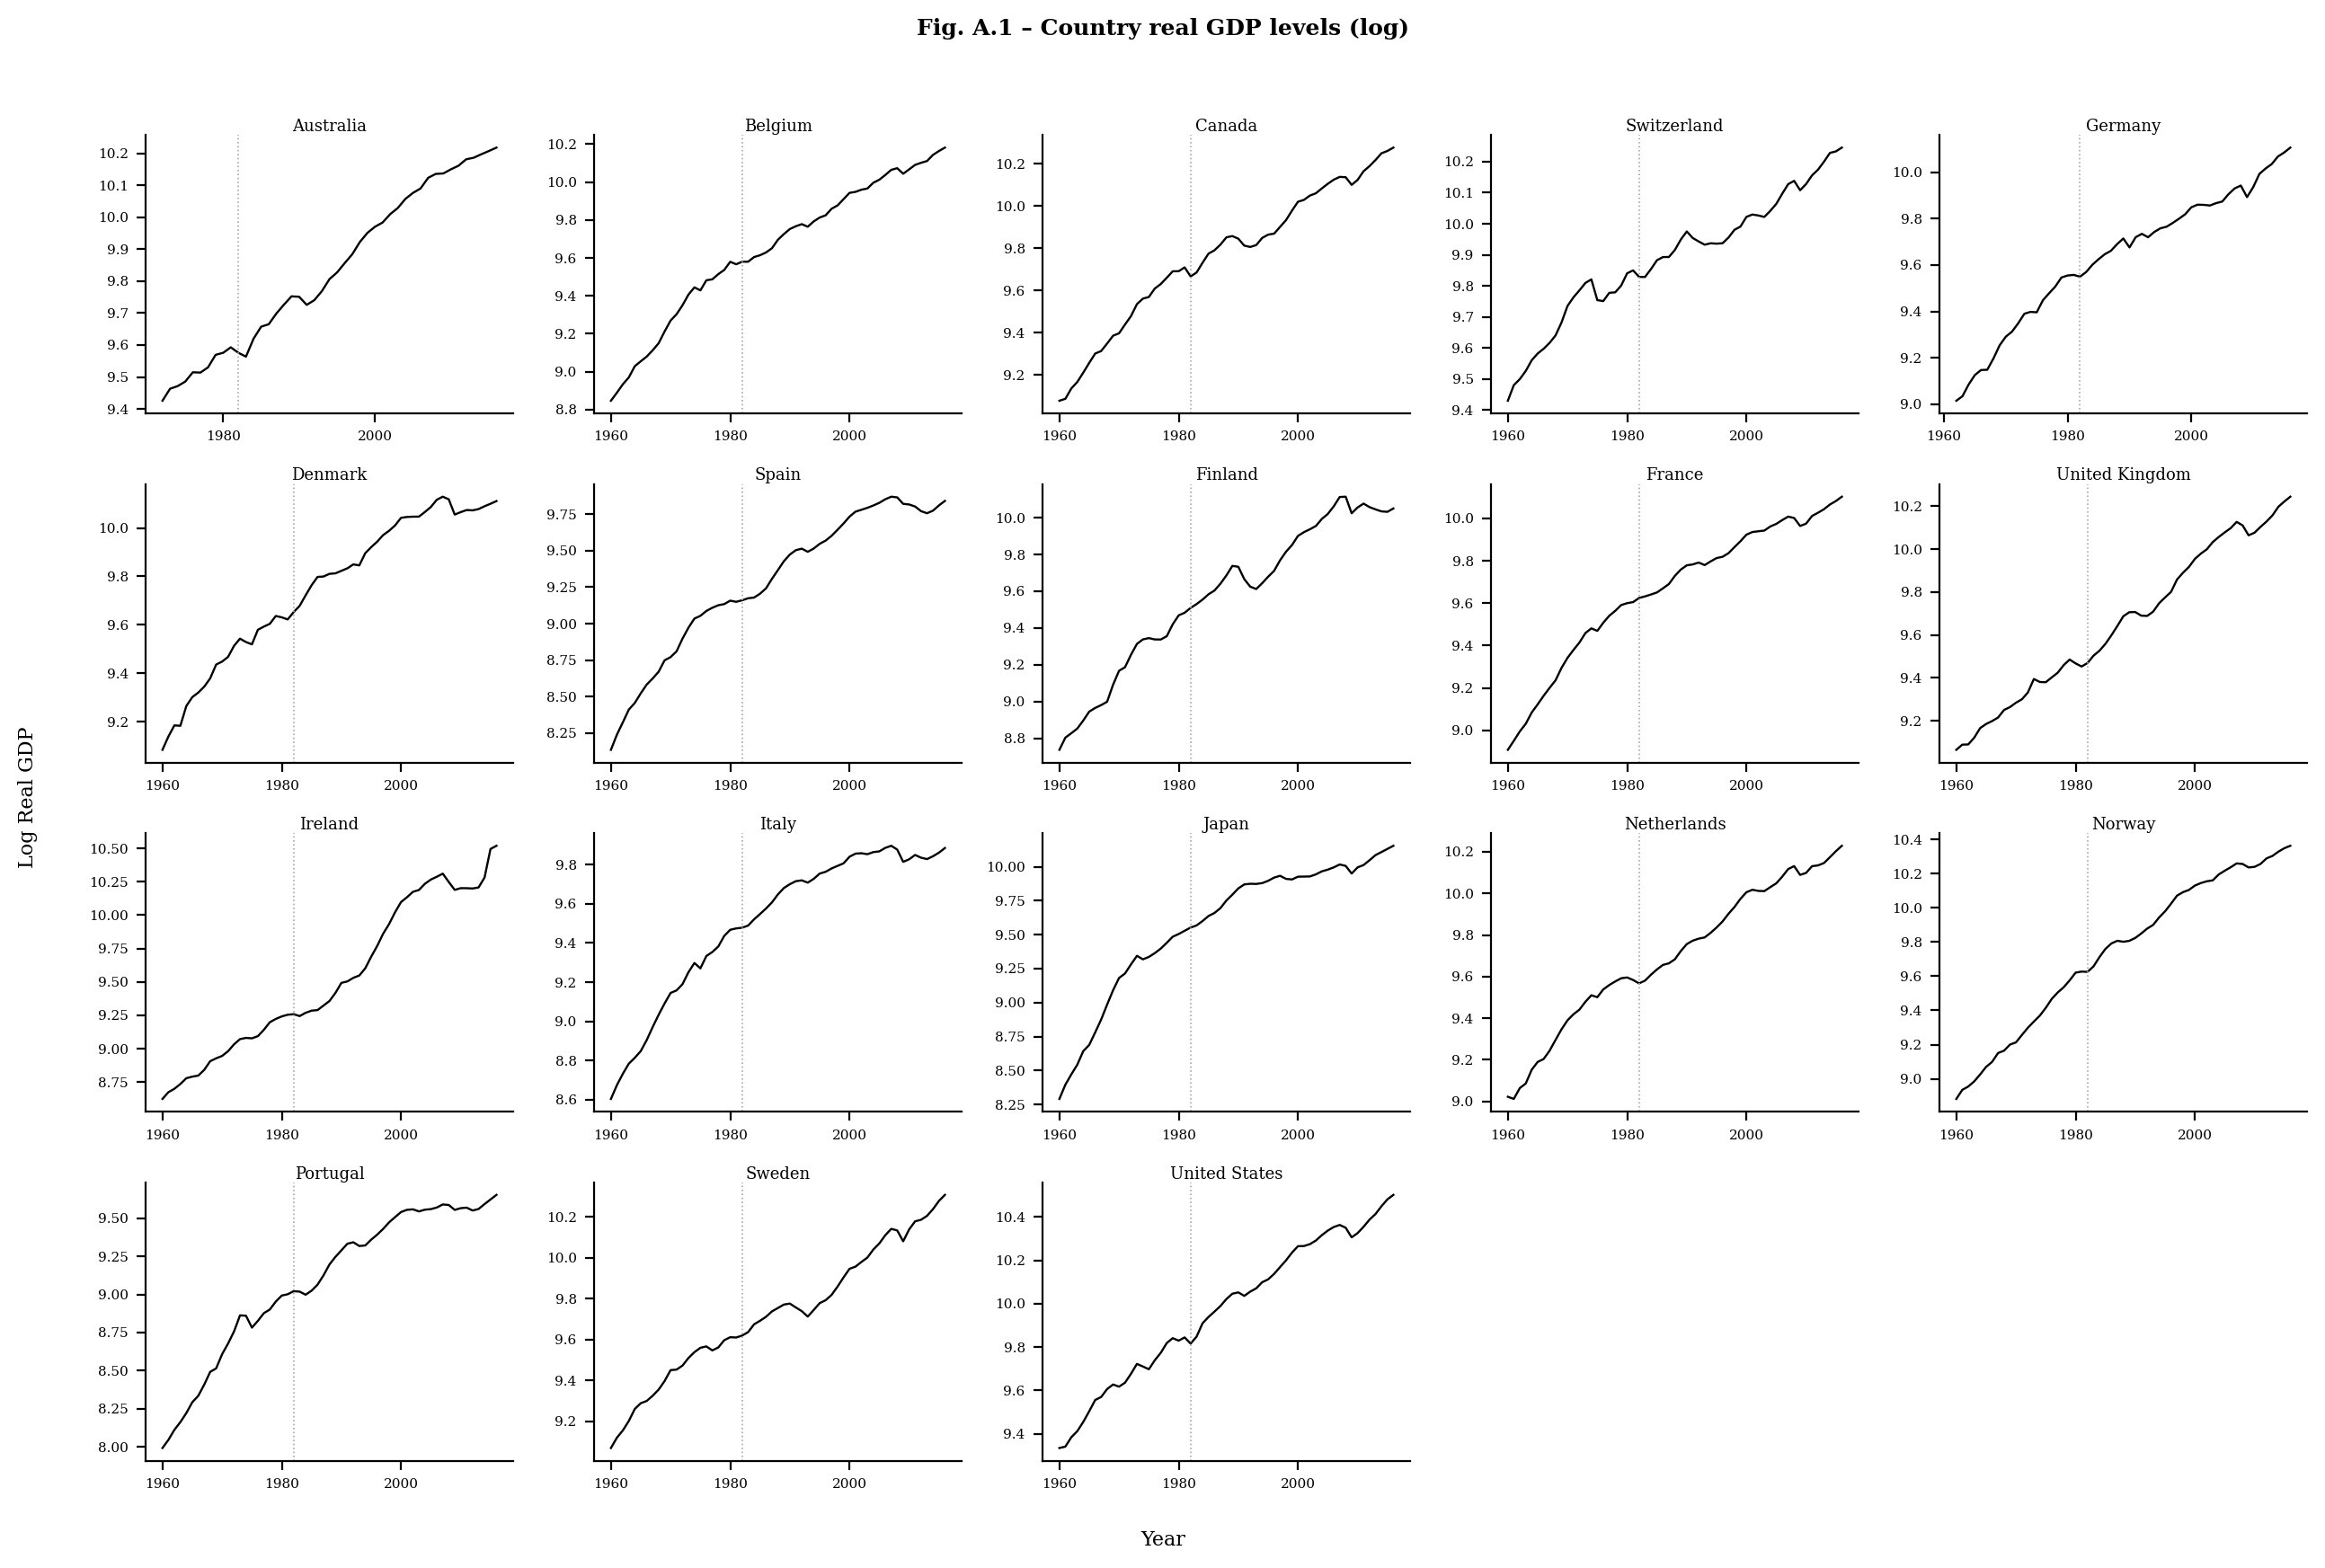
\includegraphics[width=0.95\textwidth]{outputs/figA1_gdp_levels.png}
  \caption{Fig. A1 -- GDP levels (log)}
\end{figure}

\begin{figure}[H]
  \centering
  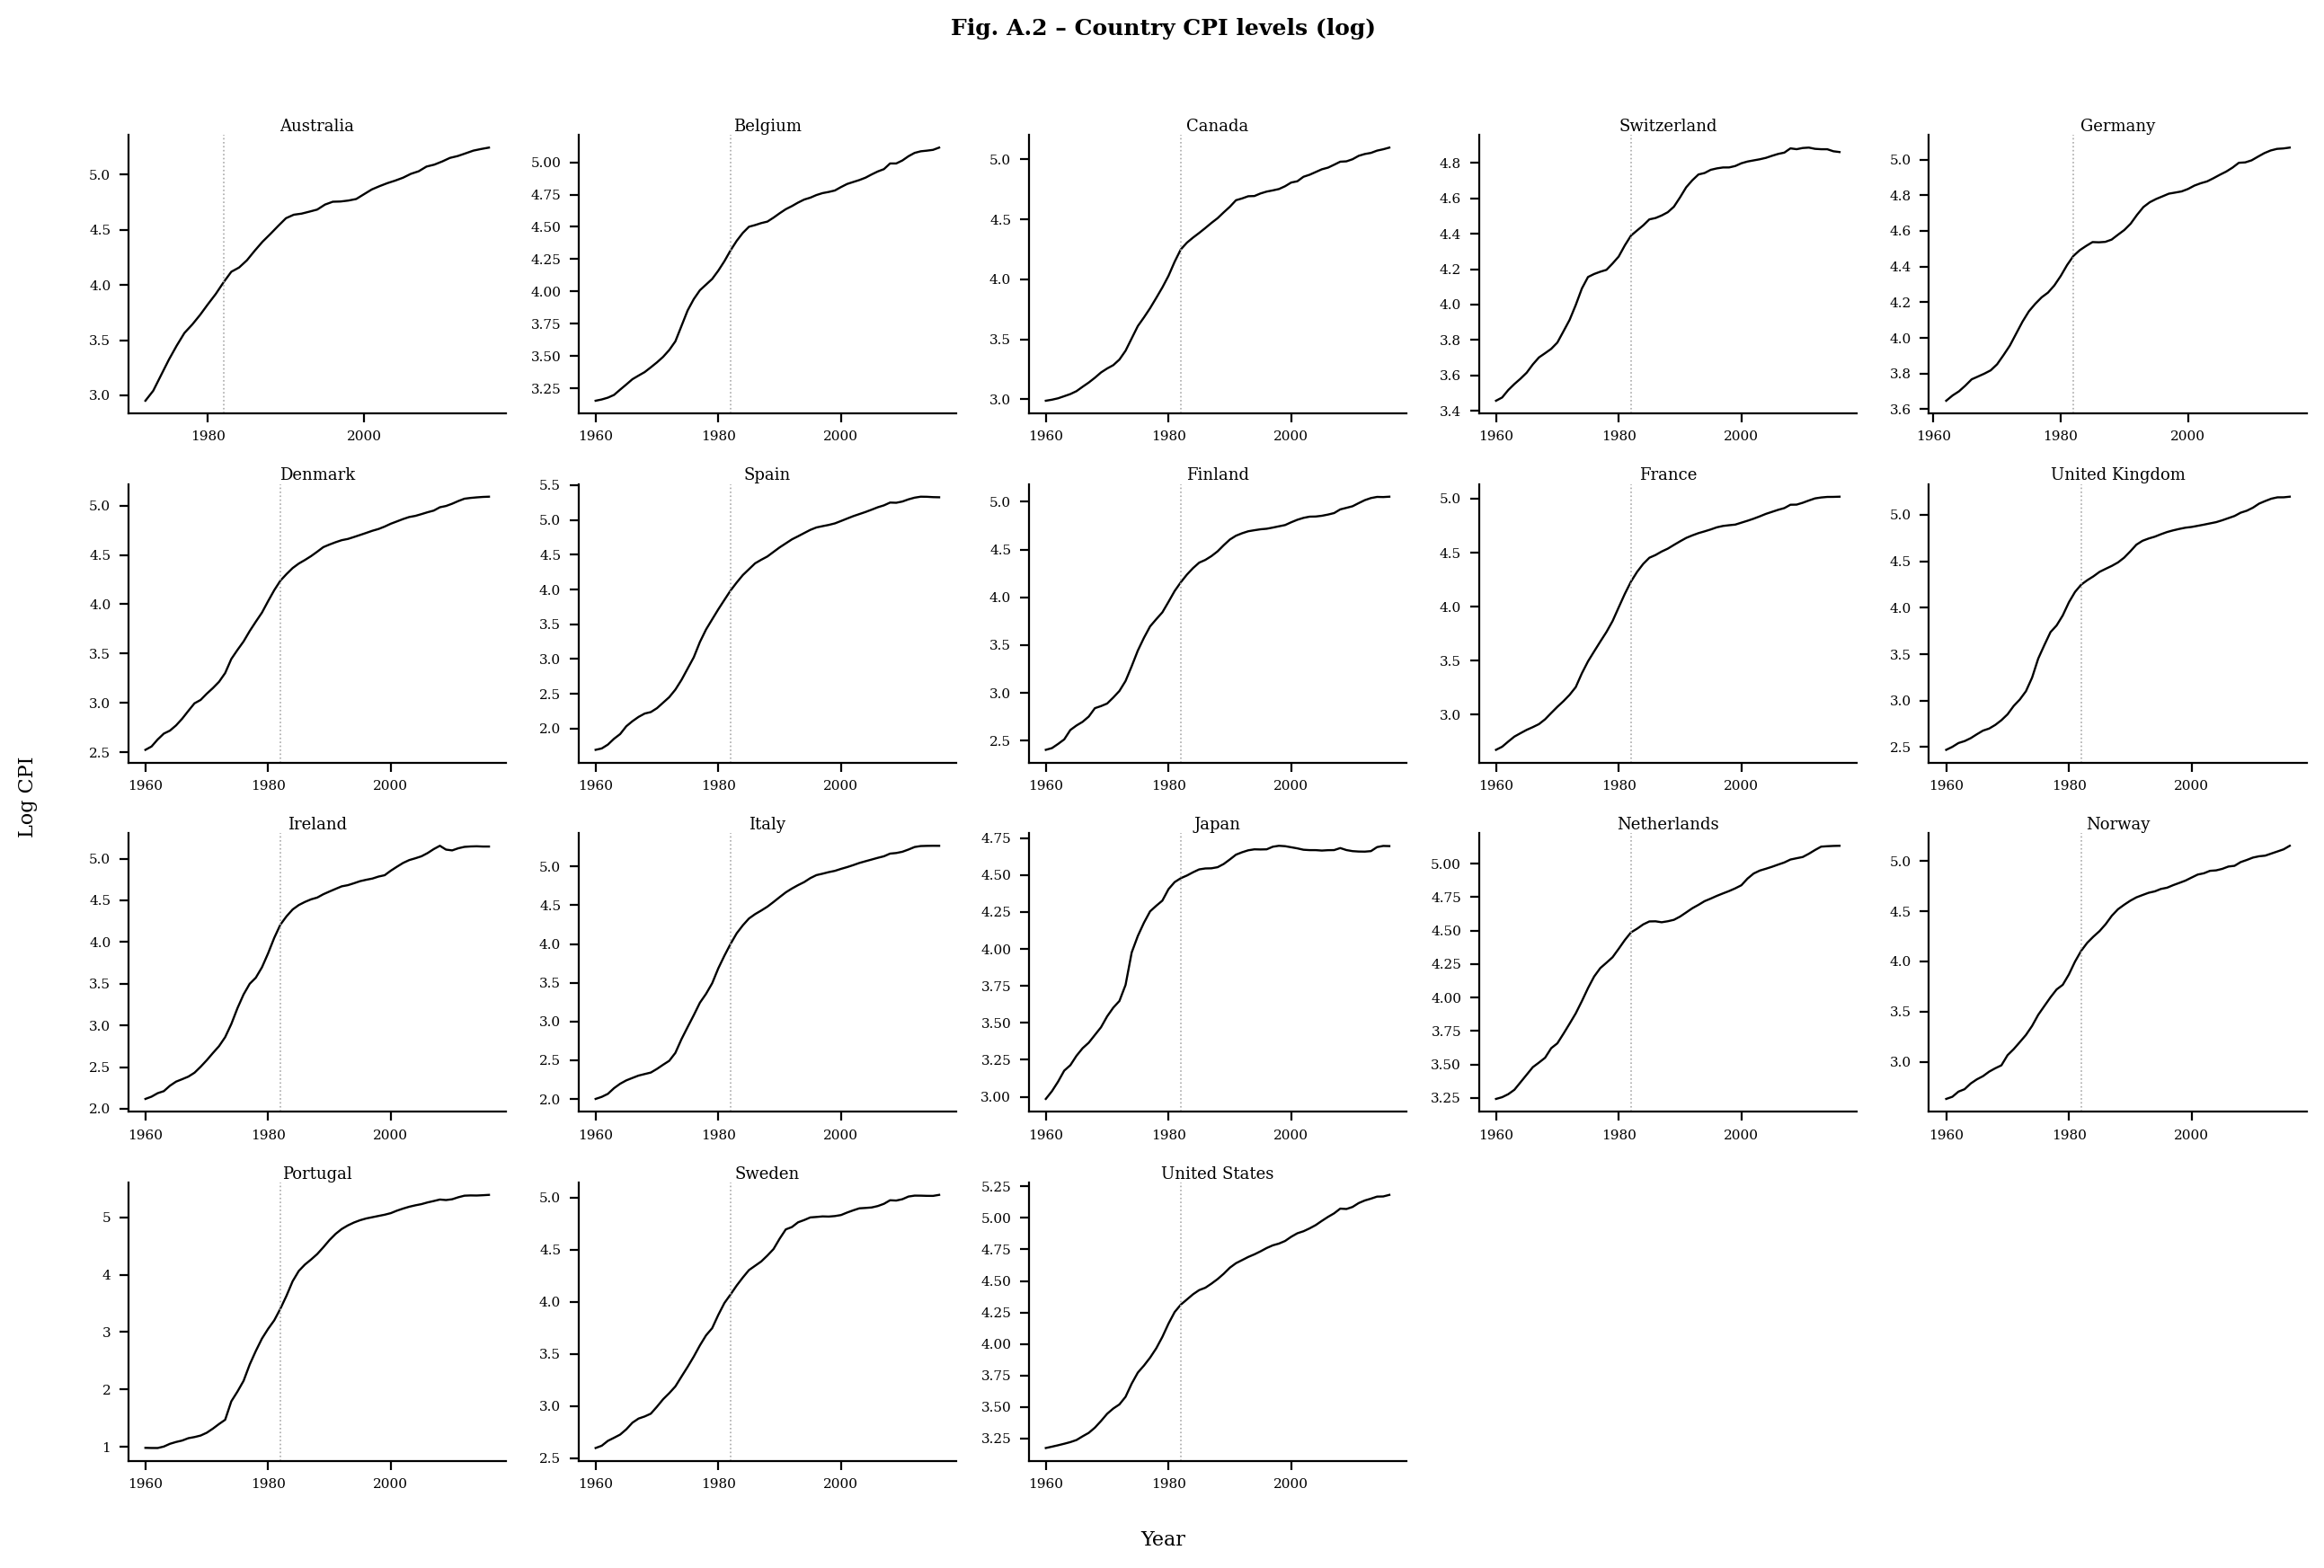
\includegraphics[width=0.95\textwidth]{outputs/figA2_cpi_levels.png}
  \caption{Fig. A2 -- CPI levels (log)}
\end{figure}

\begin{figure}[H]
  \centering
  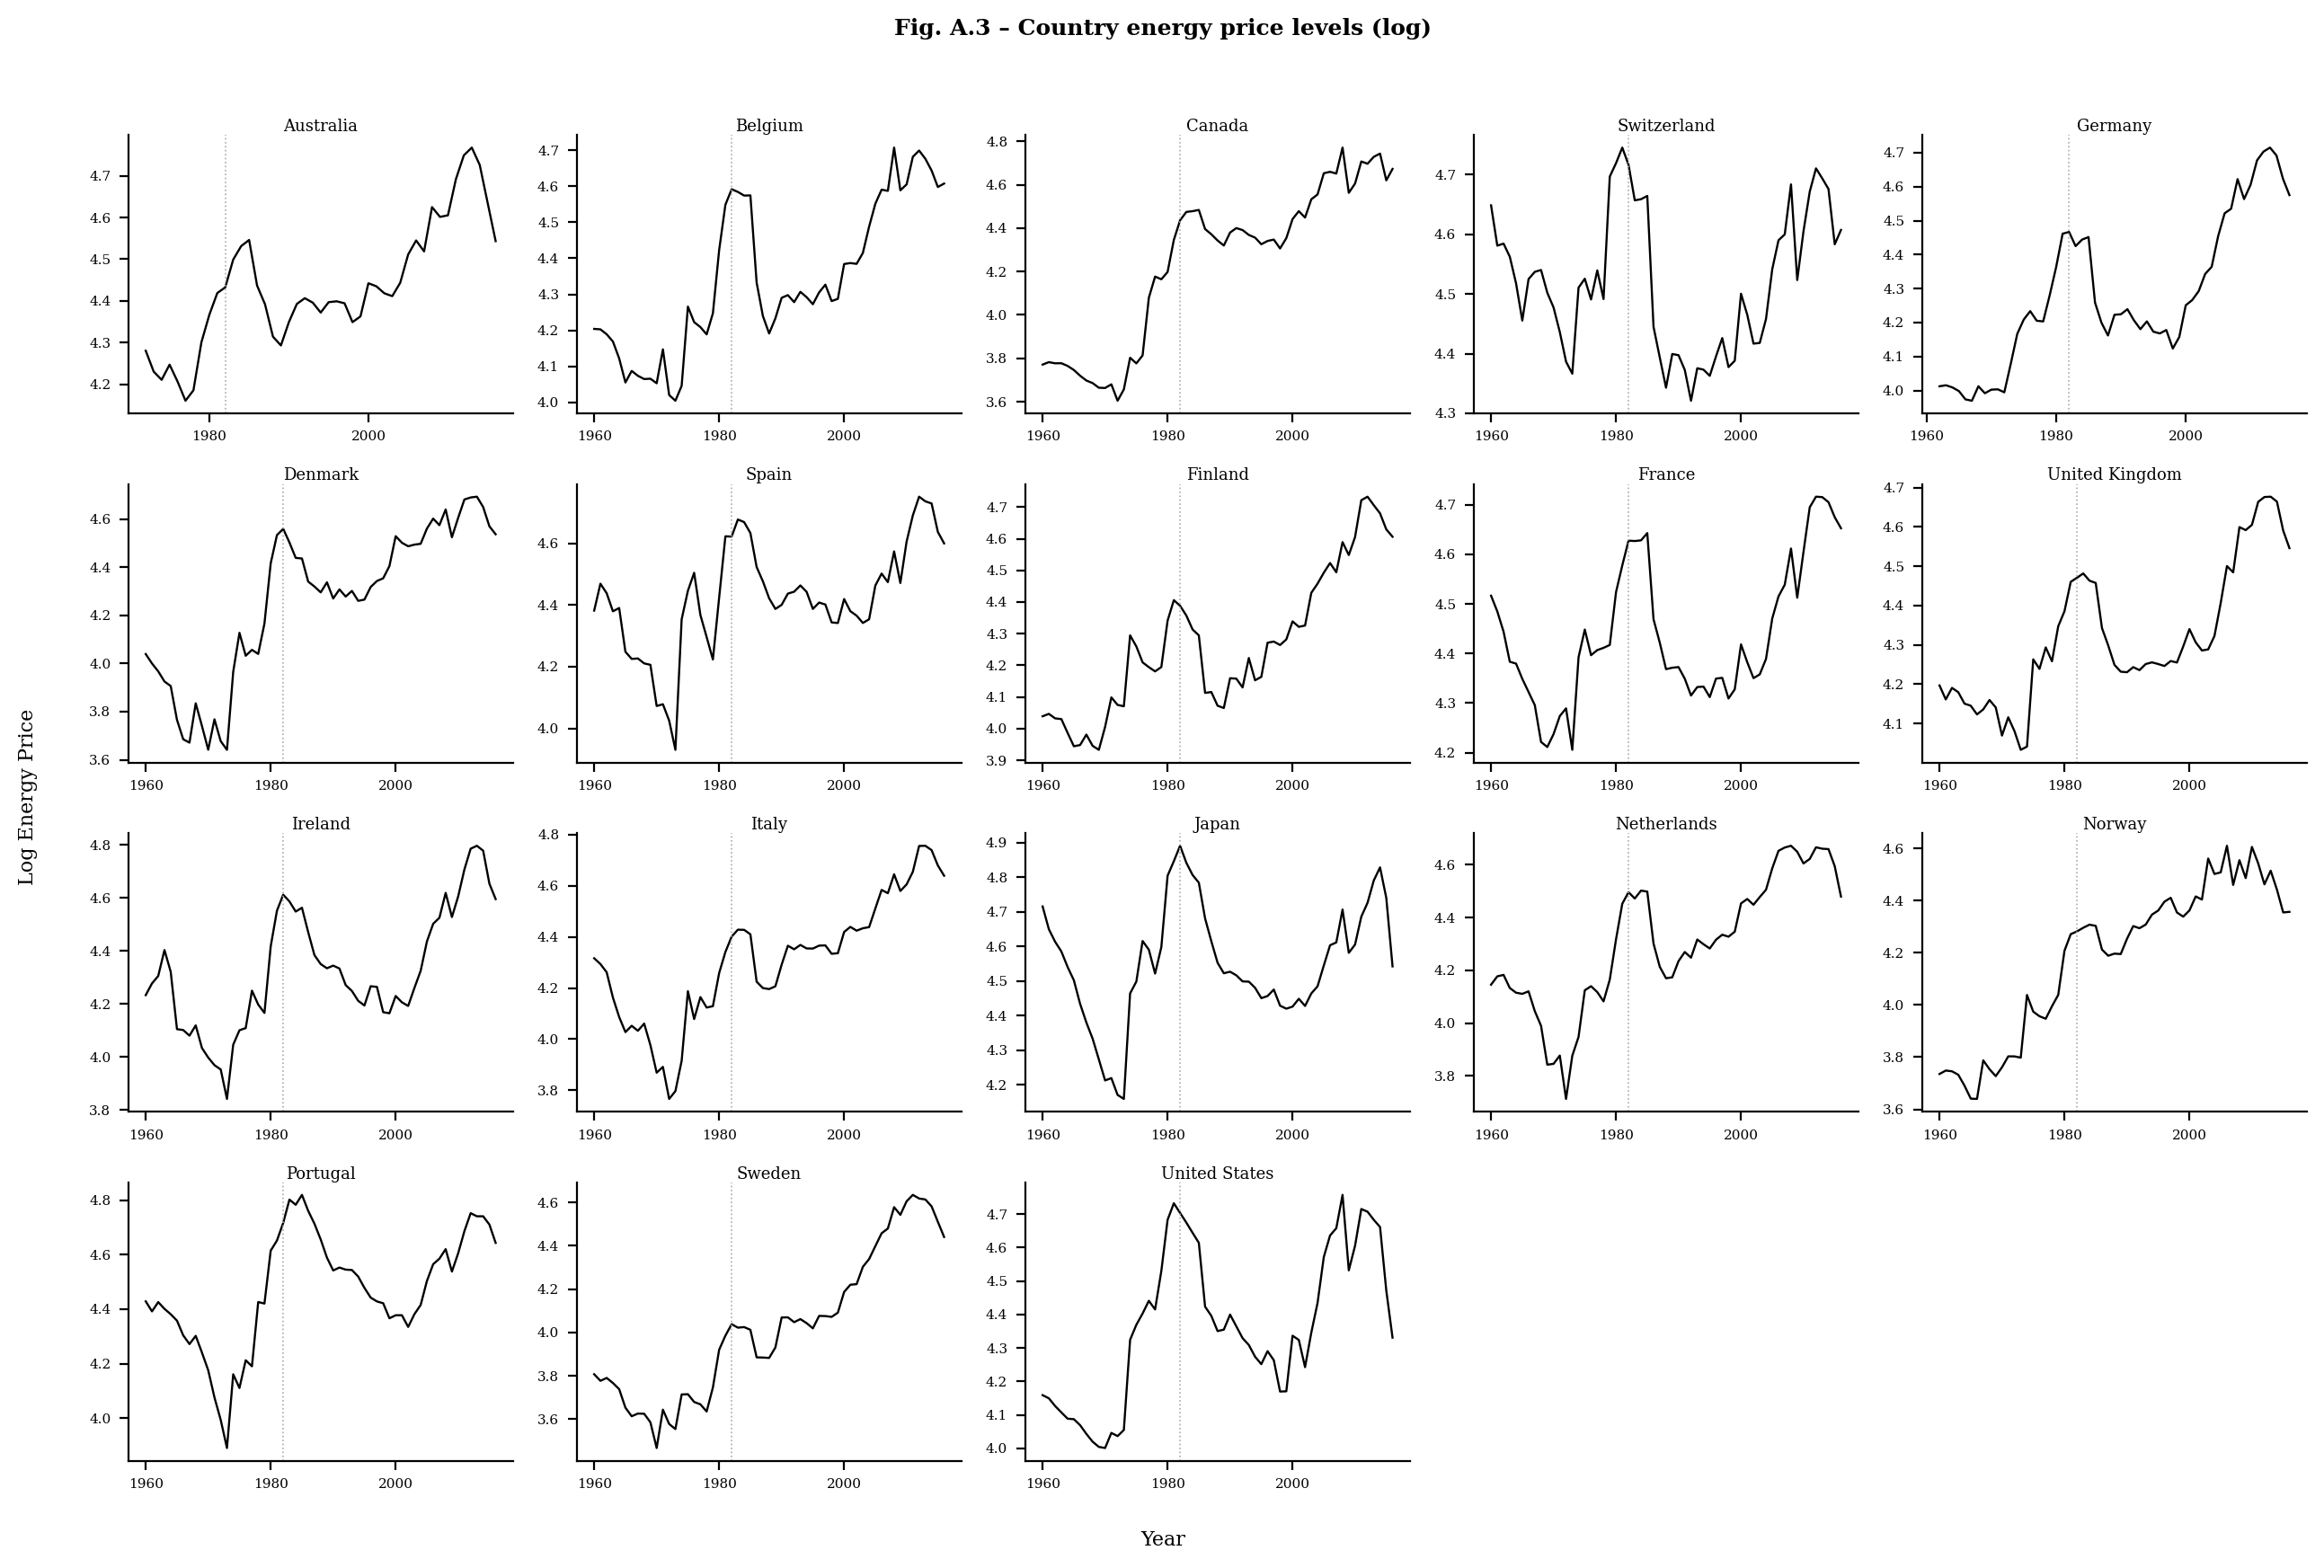
\includegraphics[width=0.95\textwidth]{outputs/figA3_energy_levels.png}
  \caption{Fig. A3 -- Energy price levels (log)}
\end{figure}

\begin{figure}[H]
  \centering
  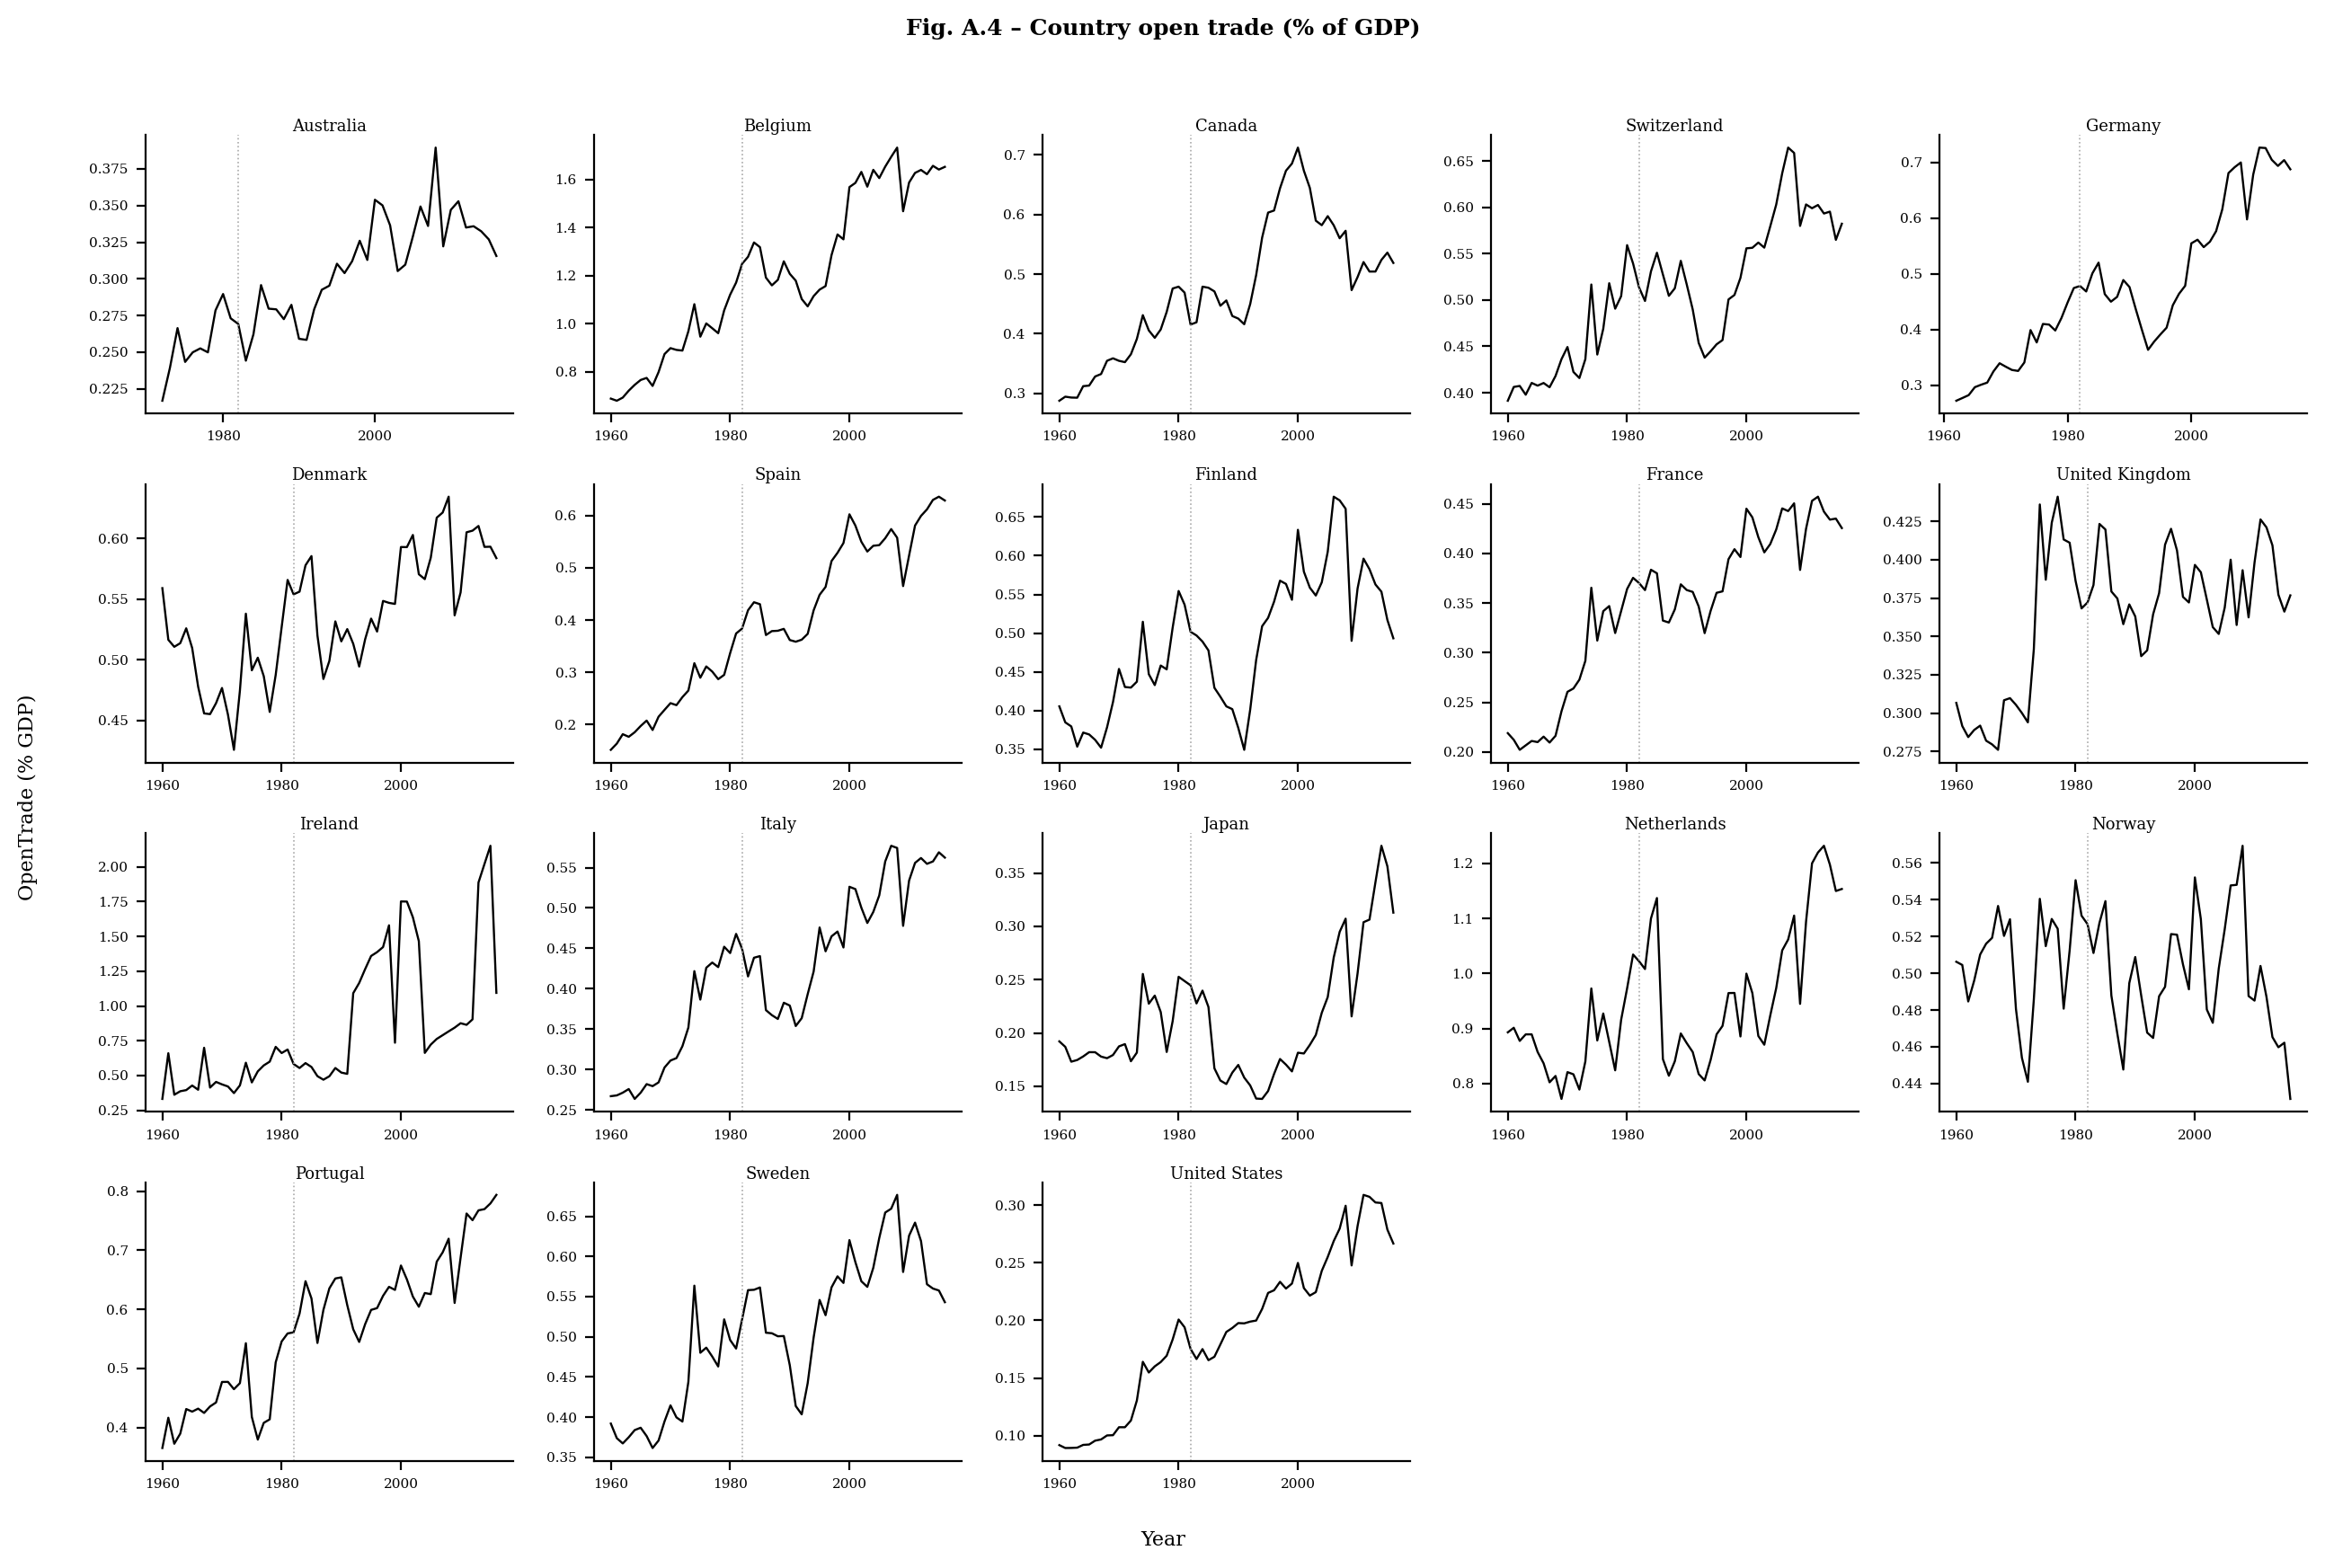
\includegraphics[width=0.95\textwidth]{outputs/figA4_opentrade.png}
  \caption{Fig. A4 -- Open trade ratio}
\end{figure}

\begin{figure}[H]
  \centering
  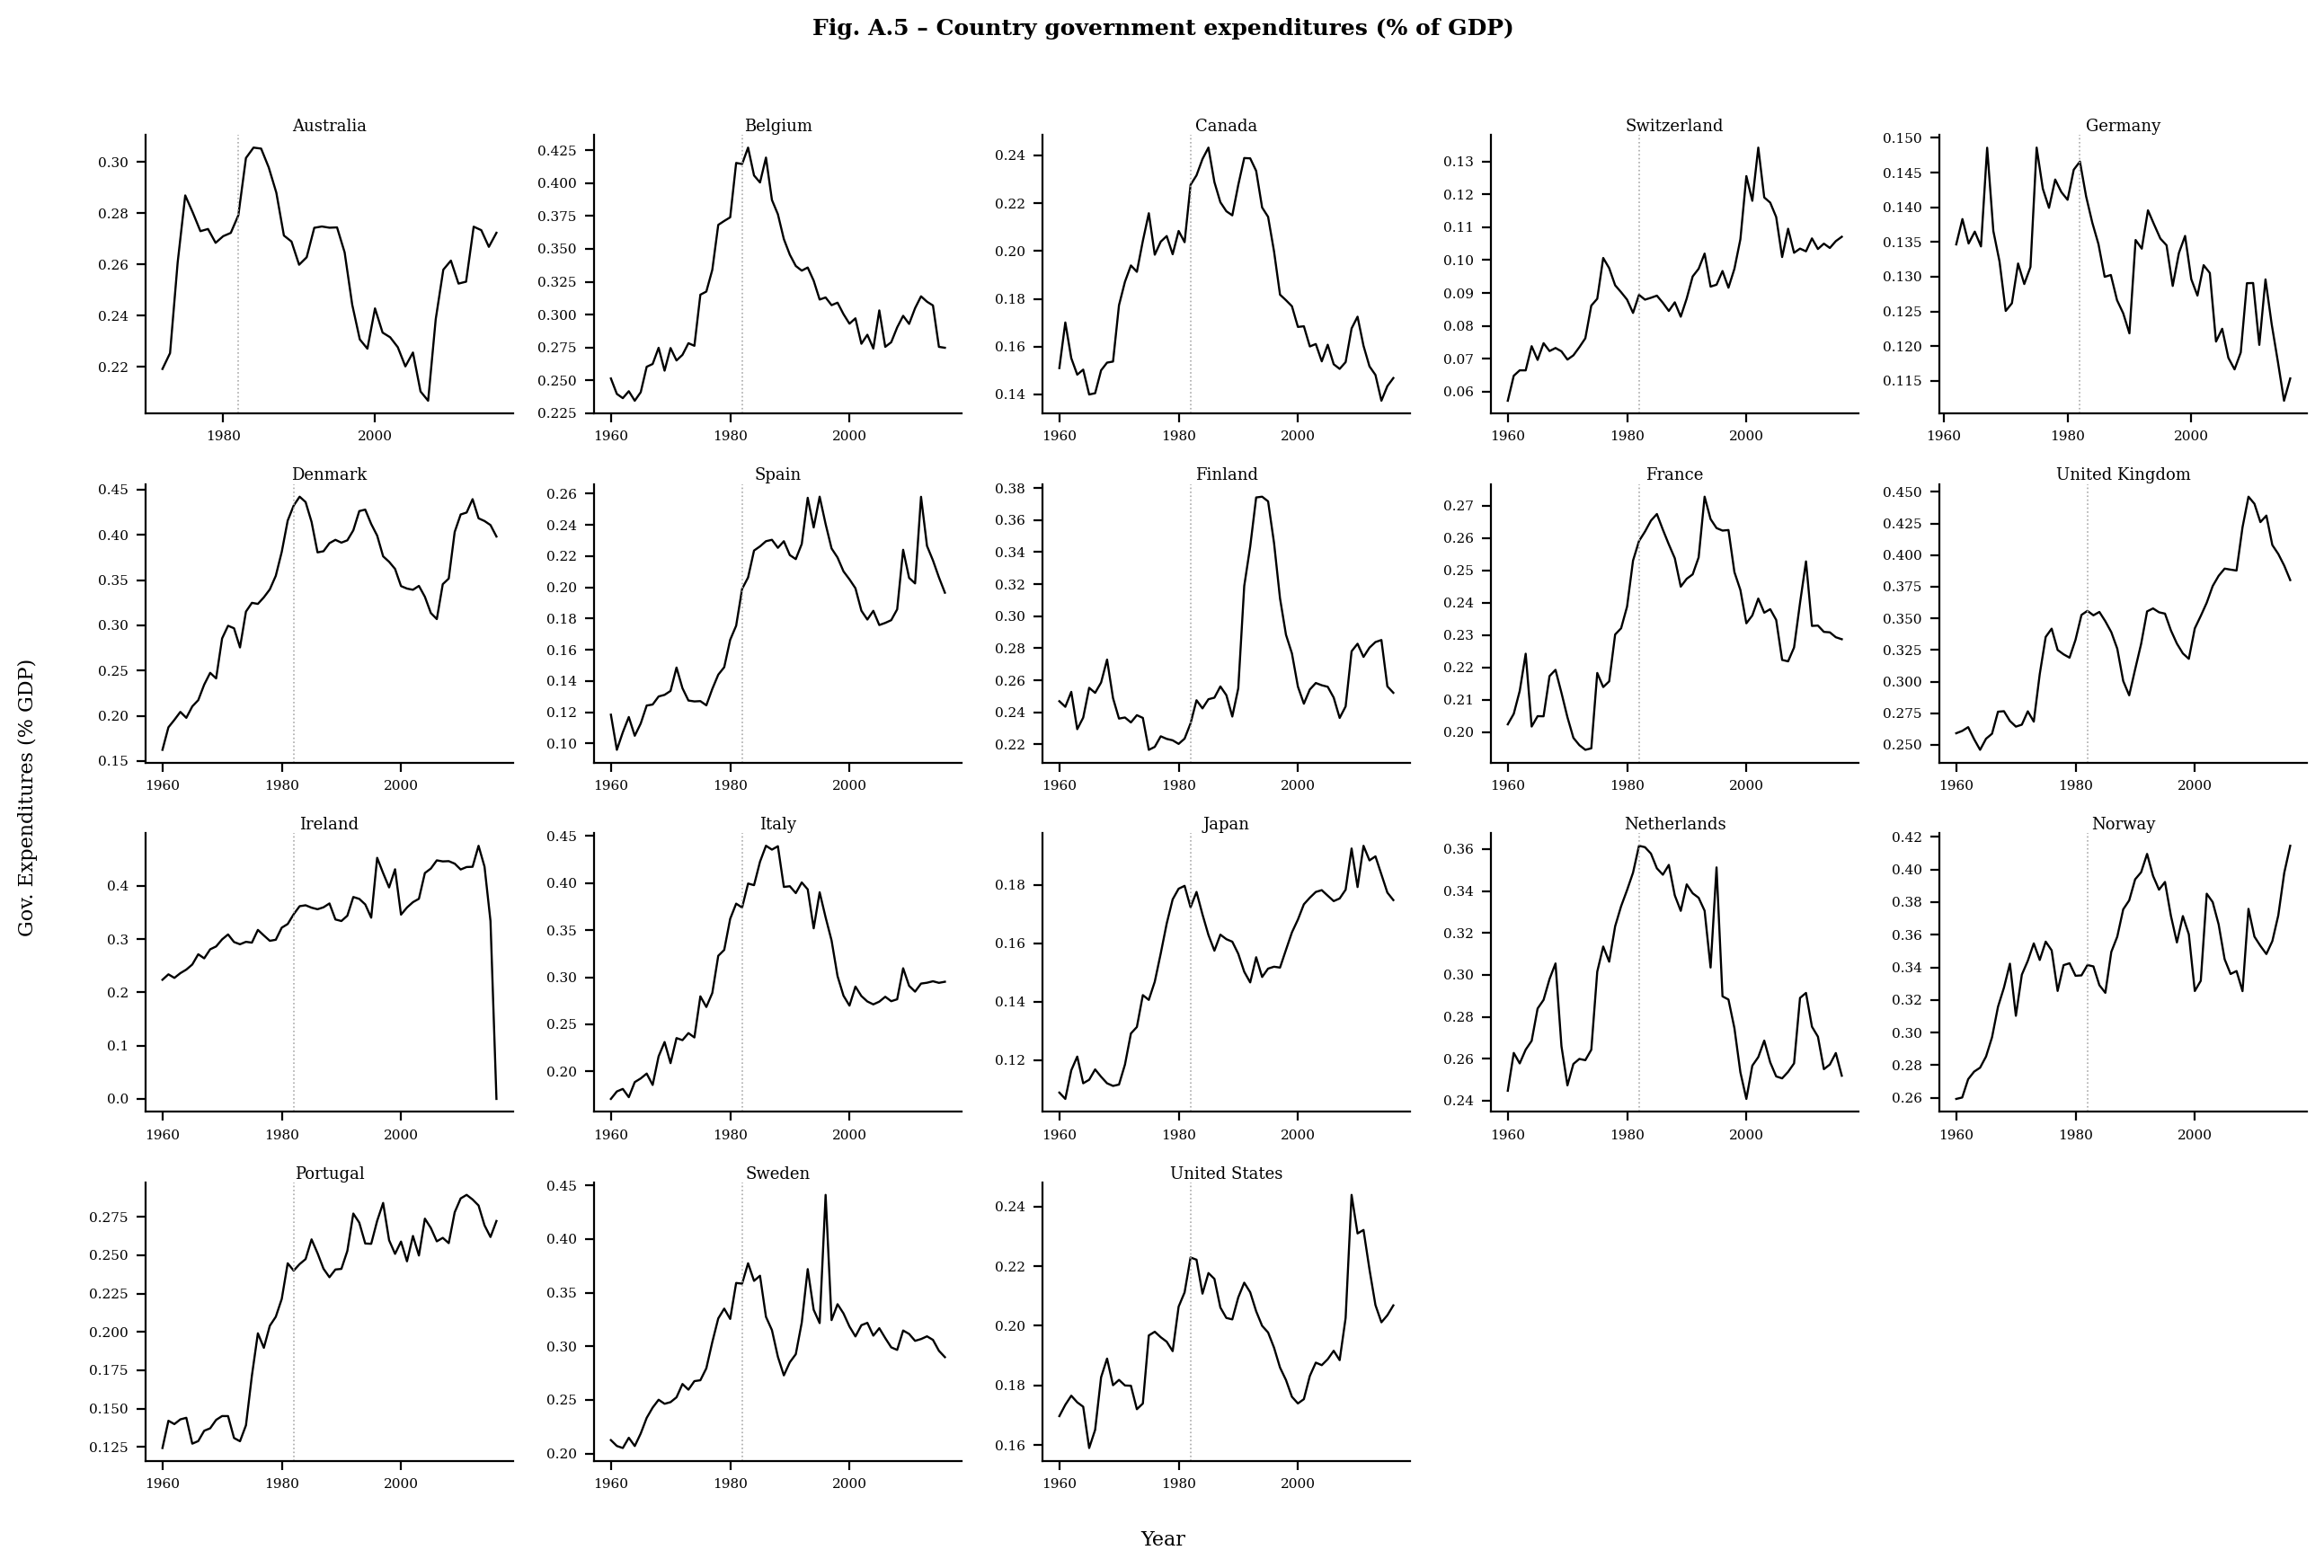
\includegraphics[width=0.95\textwidth]{outputs/figA5_govexp.png}
  \caption{Fig. A5 -- Government expenditure ratio}
\end{figure}

\begin{figure}[H]
  \centering
  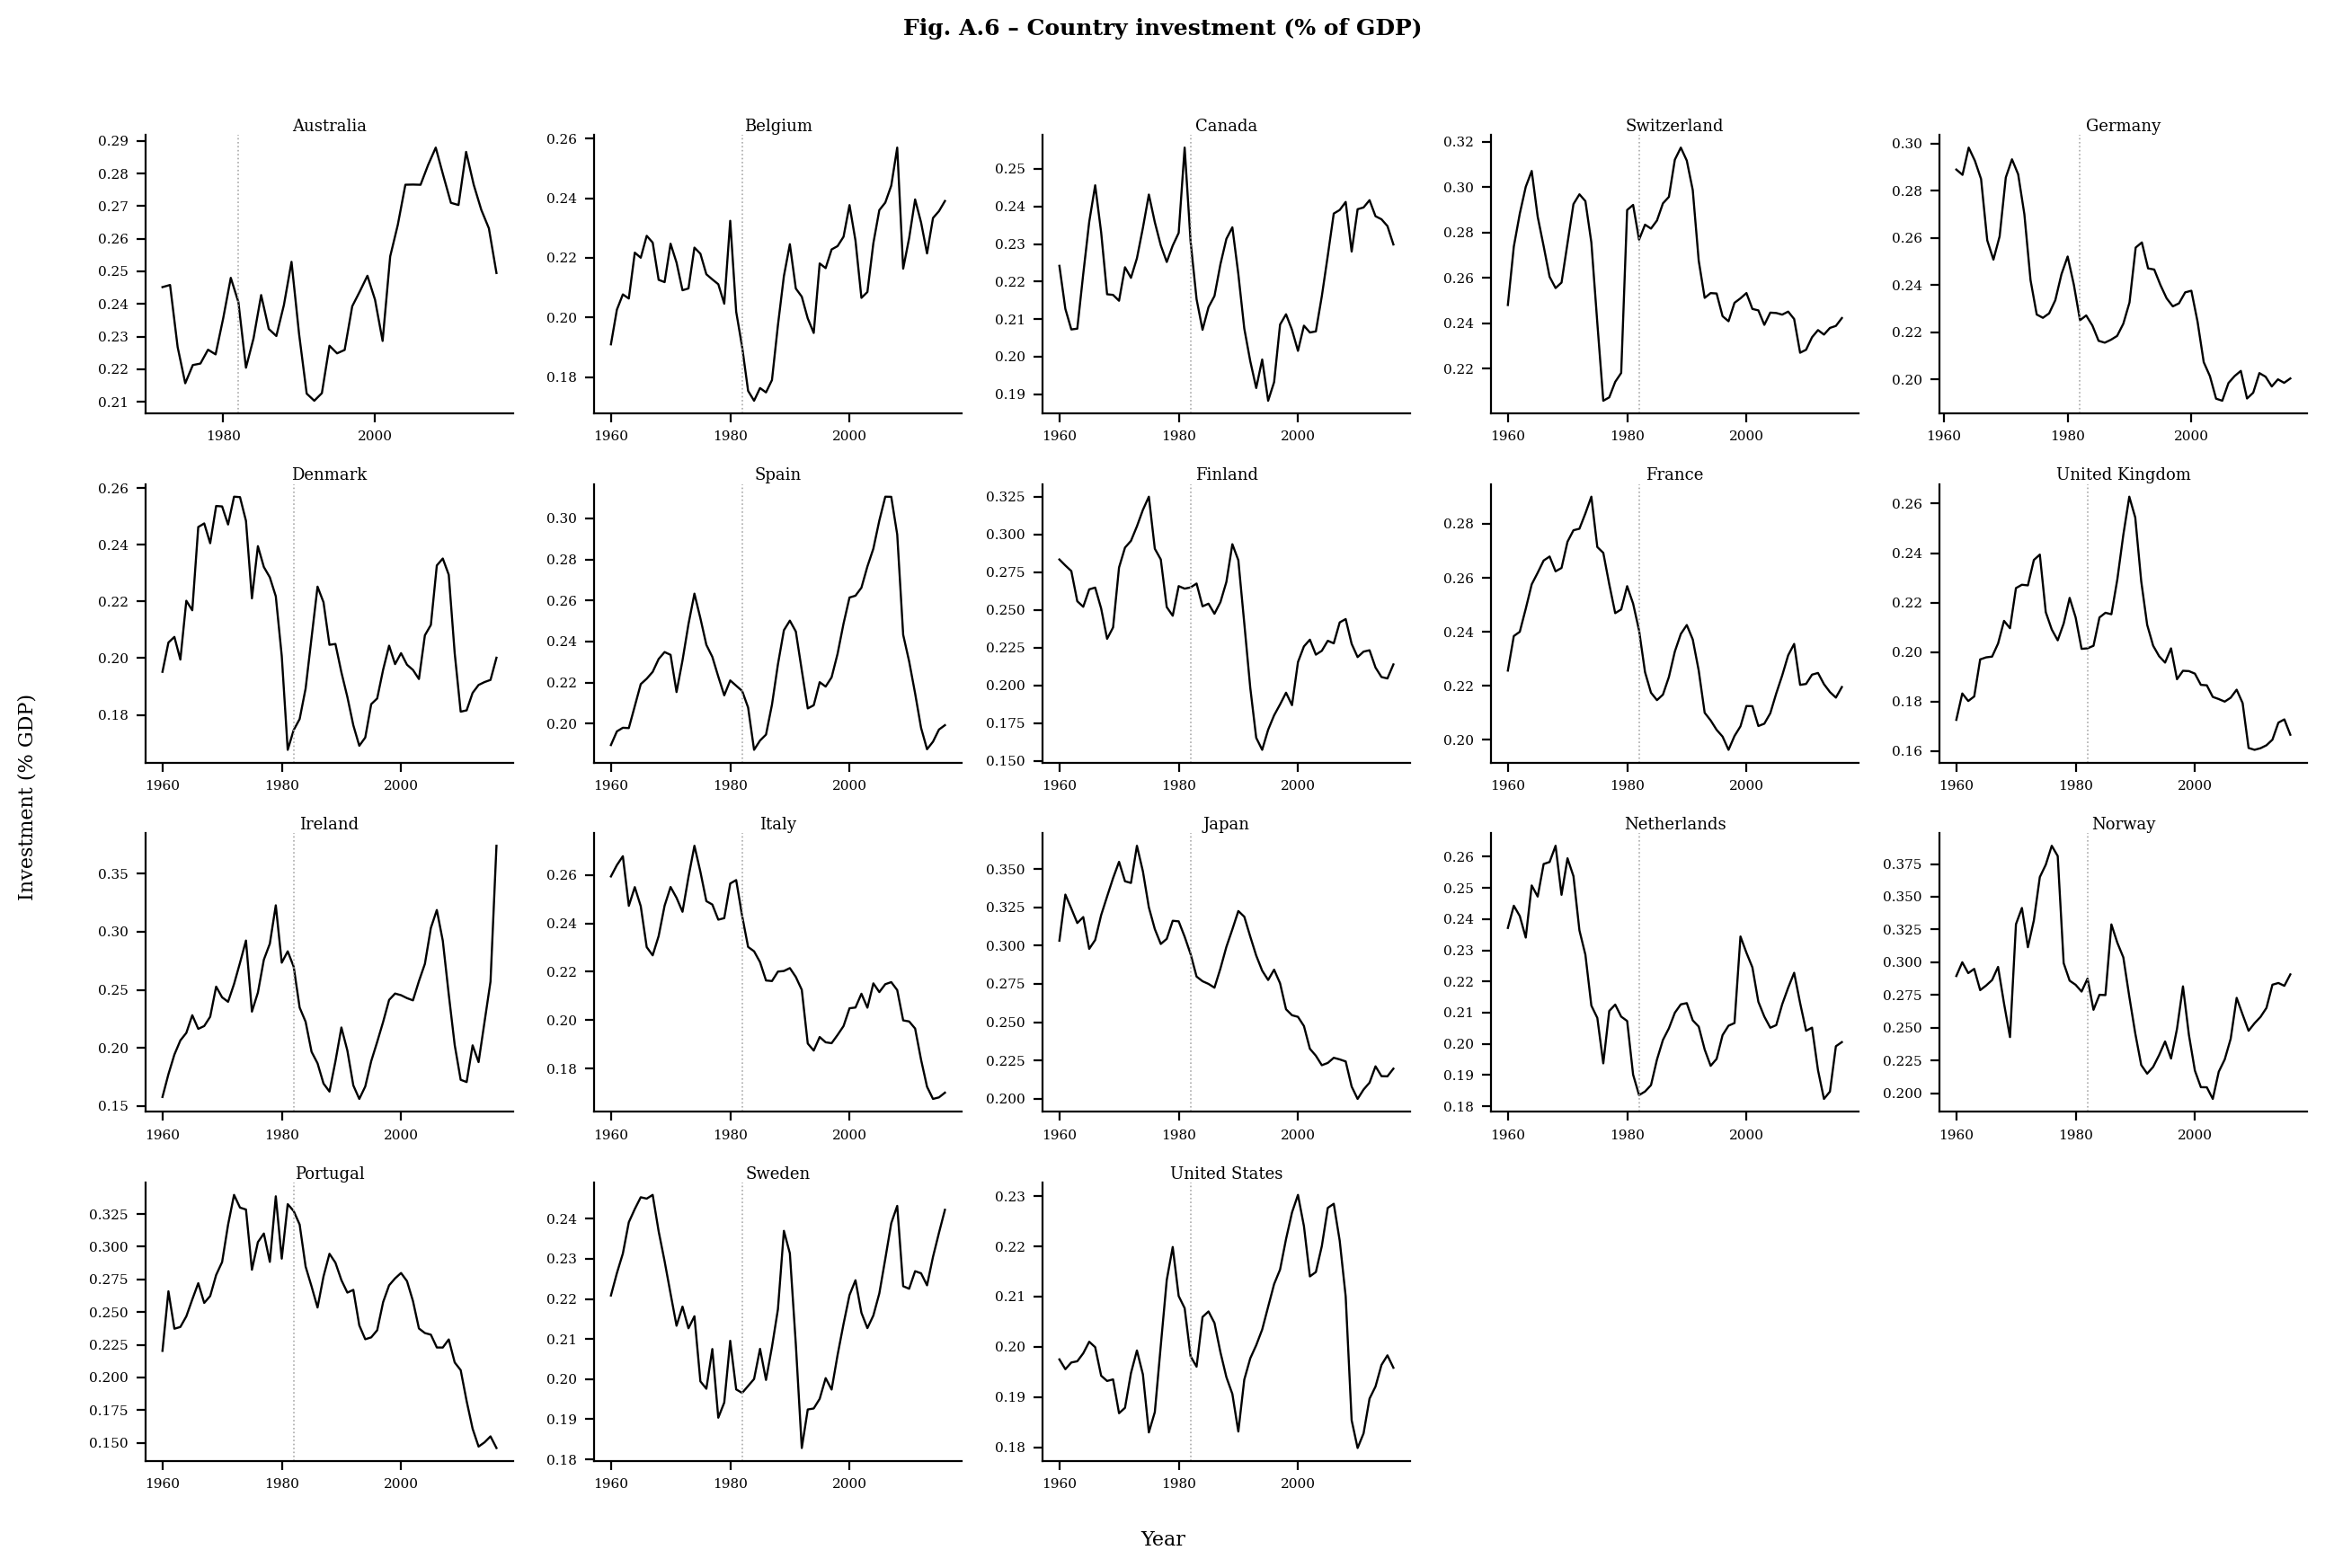
\includegraphics[width=0.95\textwidth]{outputs/figA6_investment.png}
  \caption{Fig. A6 -- Investment ratio}
\end{figure}

\begin{figure}[H]
  \centering
  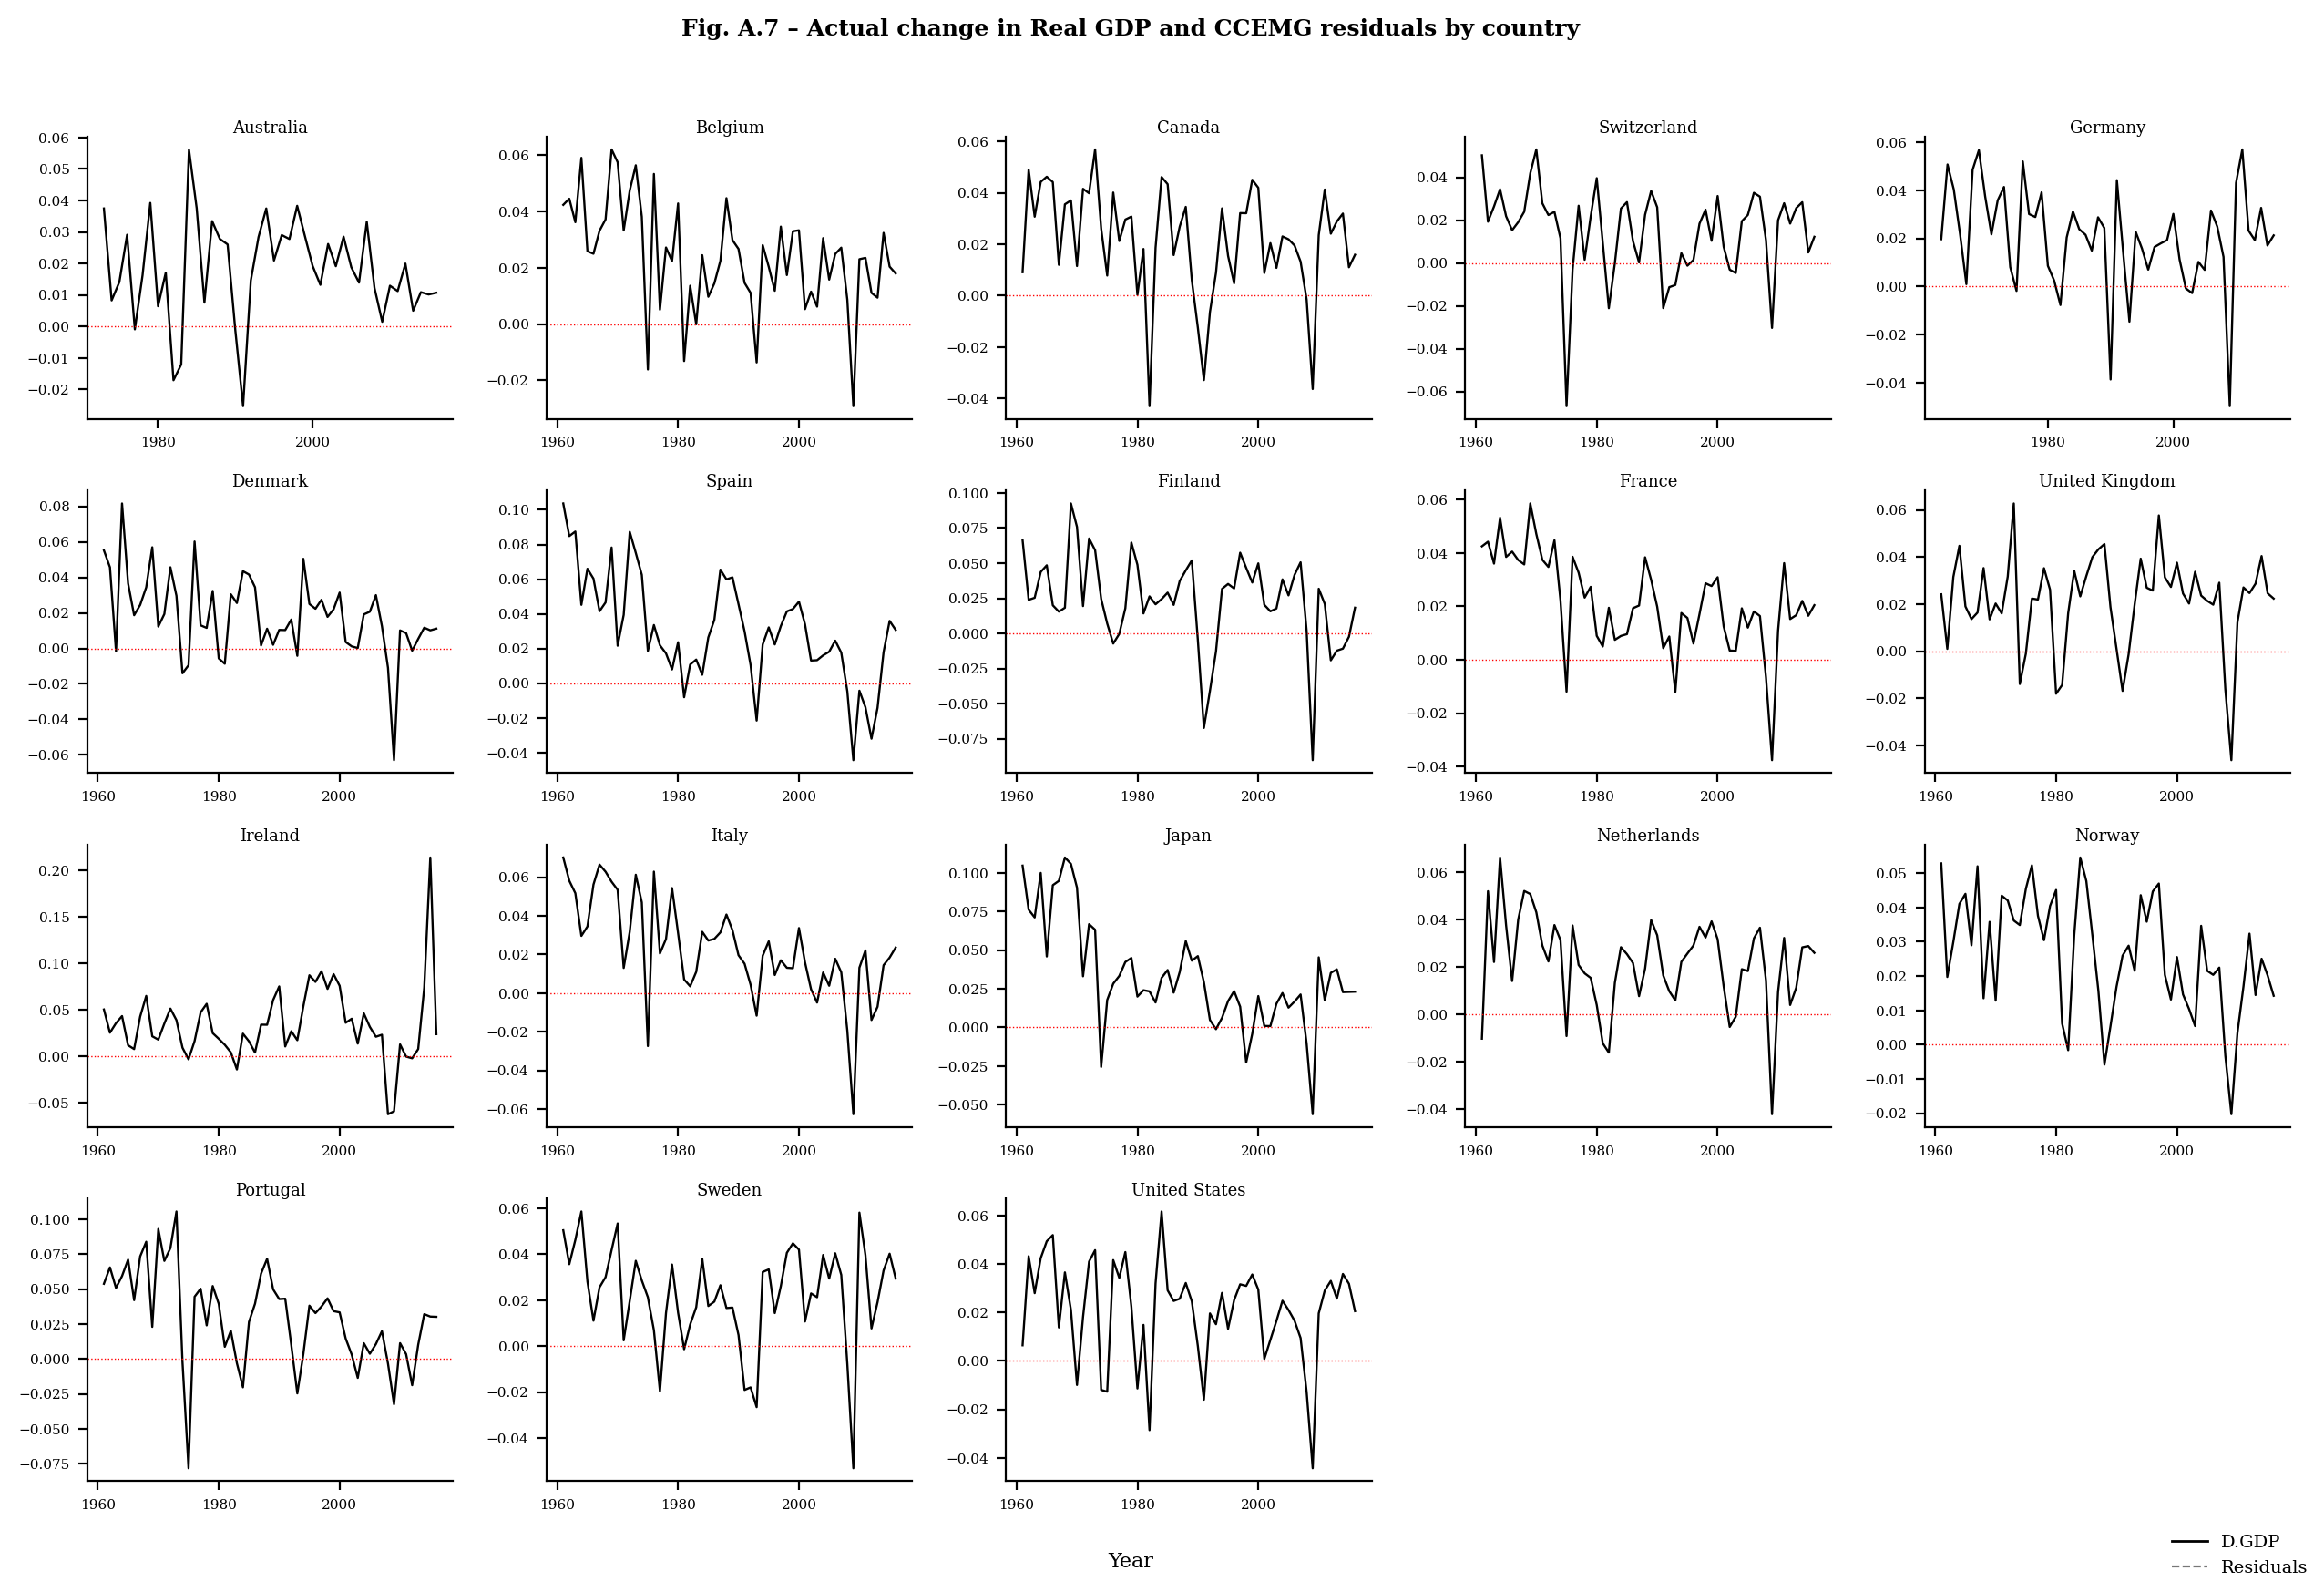
\includegraphics[width=0.95\textwidth]{outputs/figA7_gdp_residuals.png}
  \caption{Fig. A7 -- GDP growth and residuals}
\end{figure}

\section*{Optional and additional estimates}
No additional exploratory models beyond the paper were added in this version. This section can be extended with subgroup estimates or alternative functional forms if needed.

\section*{To-do list for next panel data study}
\begin{longtable}{lp{0.8\textwidth}}
\toprule
Tick & Items \\
\midrule
\endhead
$\square$ & Verify data sources and update dates before any cleaning. \\
$\square$ & Build a reproducible data pipeline with raw and processed datasets. \\
$\square$ & Inspect missingness and define the panel sample selection rules. \\
$\square$ & Compute between/within variance shares and classify variables. \\
$\square$ & Produce descriptive plots for levels, within, between, and first differences. \\
$\square$ & Run stationarity and cross-section dependence tests early. \\
$\square$ & Estimate baseline FE/RE/FD models and check multicollinearity. \\
$\square$ & Test dynamic specifications and instrument strength. \\
$\square$ & Perform robustness checks (subsamples, outliers, policy periods). \\
$\square$ & Document all code and results with a clear narrative.
\bottomrule
\end{longtable}

\end{document}
